\chapter{Entfaltung mit DSEA}

% MAKE MODEL
\begin{lstlisting}[language=Python, basicstyle=\small, captionpos=b, caption=Die Funktion wird zu Erstellung des Modells verwendet. Hier wird das NN mithilfe der Keras-API \cite{tensorflow2015-whitepaper} definiert. Die Ebenen können beliebig angepasst und erweitert werden., label=code:model]
def make_model(num_features, num_classes, learning_rate=0.0005): 
    """
    num_features: Number of features
    num_classes: Number of energy classes
    learning_rate: Hyperparameter of the ADAM optimizer
    """
    model = tf.keras.Sequential()

    # input layer
    model.add(tf.keras.layers.Dense(120, input_shape=num_features,
    activation='relu'))
    
    # dense layer
    model.add(tf.keras.layers.Dense(240, activation='relu'))
    model.add(tf.keras.layers.Dense(120, activation='relu'))
    model.add(tf.keras.layers.Dense(12, activation='relu'))
    
    # output layer
    model.add(tf.keras.layers.Dense(num_classes, activation='softmax'))

    # define optimizer, loss function and metric
    opt = tf.keras.optimizers.Adam(learning_rate=learning_rate)
    loss = tf.keras.losses.CategoricalCrossentropy()
    acc = tf.keras.metrics.CategoricalAccuracy(
        name="categorical_accuracy", dtype=None)

    # compile the tensorflow model
    model.compile(optimizer=opt, loss=loss, metrics=[acc, chi2])

    return model
\end{lstlisting}

\newpage
% WRAPPER
\begin{lstlisting}[language=Python, basicstyle=\small, captionpos=b, caption=Quellcode des Wrappers zur Verwendung der Keras-API\cite{tensorflow2015-whitepaper} in DSEA. Es wird die Funktion \textbf{make\_model} im Anhang \ref{code:model} zur Erstellung der Tensorflow-Modelle benötigt., label=code:wrapper]
class MyClassifier():
    """
    Parameters
    ---------
    one_model: bool
        If True, dsea will train only one model instead of 
        generating a new one in each dsea iteration
    batch_size: int
        Split data into batches with the size of batch_size
    epochs: int
        Number of epochs
    learning_rate: float
        Stepsize of the optimizer ADAM
    """

    def __init__(self, batch_size=2048, epochs=5, learning_rate=0.0005,
    one_model=True):        
        self.batch_size = batch_size
        self.epochs = epochs
        self.learning_rate = learning_rate
        self.one_model = one_model
        self.model = None #tensorflow model if created
        self.Niter = 0 #current DSEA iteration
        self.history = [] #model history for each dsea iteration

    def fit(self, X, y, sample_weight=None):
        # train self.model on weighted data X with label y

        # print progress
        self.Niter += 1
        print(f'\nNumber iteration in DSEA: {self.Niter}')

        # y is NOT one-hot encoded yet
        y_hot = np.zeros((y.size, y.max()+1))
        y_hot[np.arange(y.size),y] = 1
        
        # create new model if (one_model=False) or
        # (one_model = True and there exist no model yet)
        if self.model is None or self.one_model is False:
            self.model = make_model(num_features=(len(feature_list), ),
            num_classes=y.max()+1, learning_rate=self.learning_rate)

        # save training history
        history = self.model.fit(X, y_hot, sample_weight=sample_weight,
        batch_size=self.batch_size, epochs=self.epochs)
        self.history.append(history)

        return self

    def predict_proba(self, X):
        # predict X, returns confidences c_ij for each row i and class j
        return self.model.predict(X)

    def get_model(self):
        # return the tensorflow model
        return self.model

    def get_model_history(self):
        # return the history of loss, accuracy and chi2 distance
        # of the training process
        list_loss = []
        list_acc = []
        list_chi = []

        # list of lists --> one list
        for history in self.history:
            list_loss += history.history['loss']
            list_acc += history.history['categorical_accuracy']
            list_chi += history.history['chi2']

        # list to numpy array
        list_loss = np.array(list_loss, dtype='float32')
        list_acc = np.array(list_acc, dtype='float32')
        list_chi = np.array(list_chi, dtype='float32')

        return list_loss, list_acc, list_chi
\end{lstlisting}

% chi2 scatter: False
\begin{figure}
    \centering
    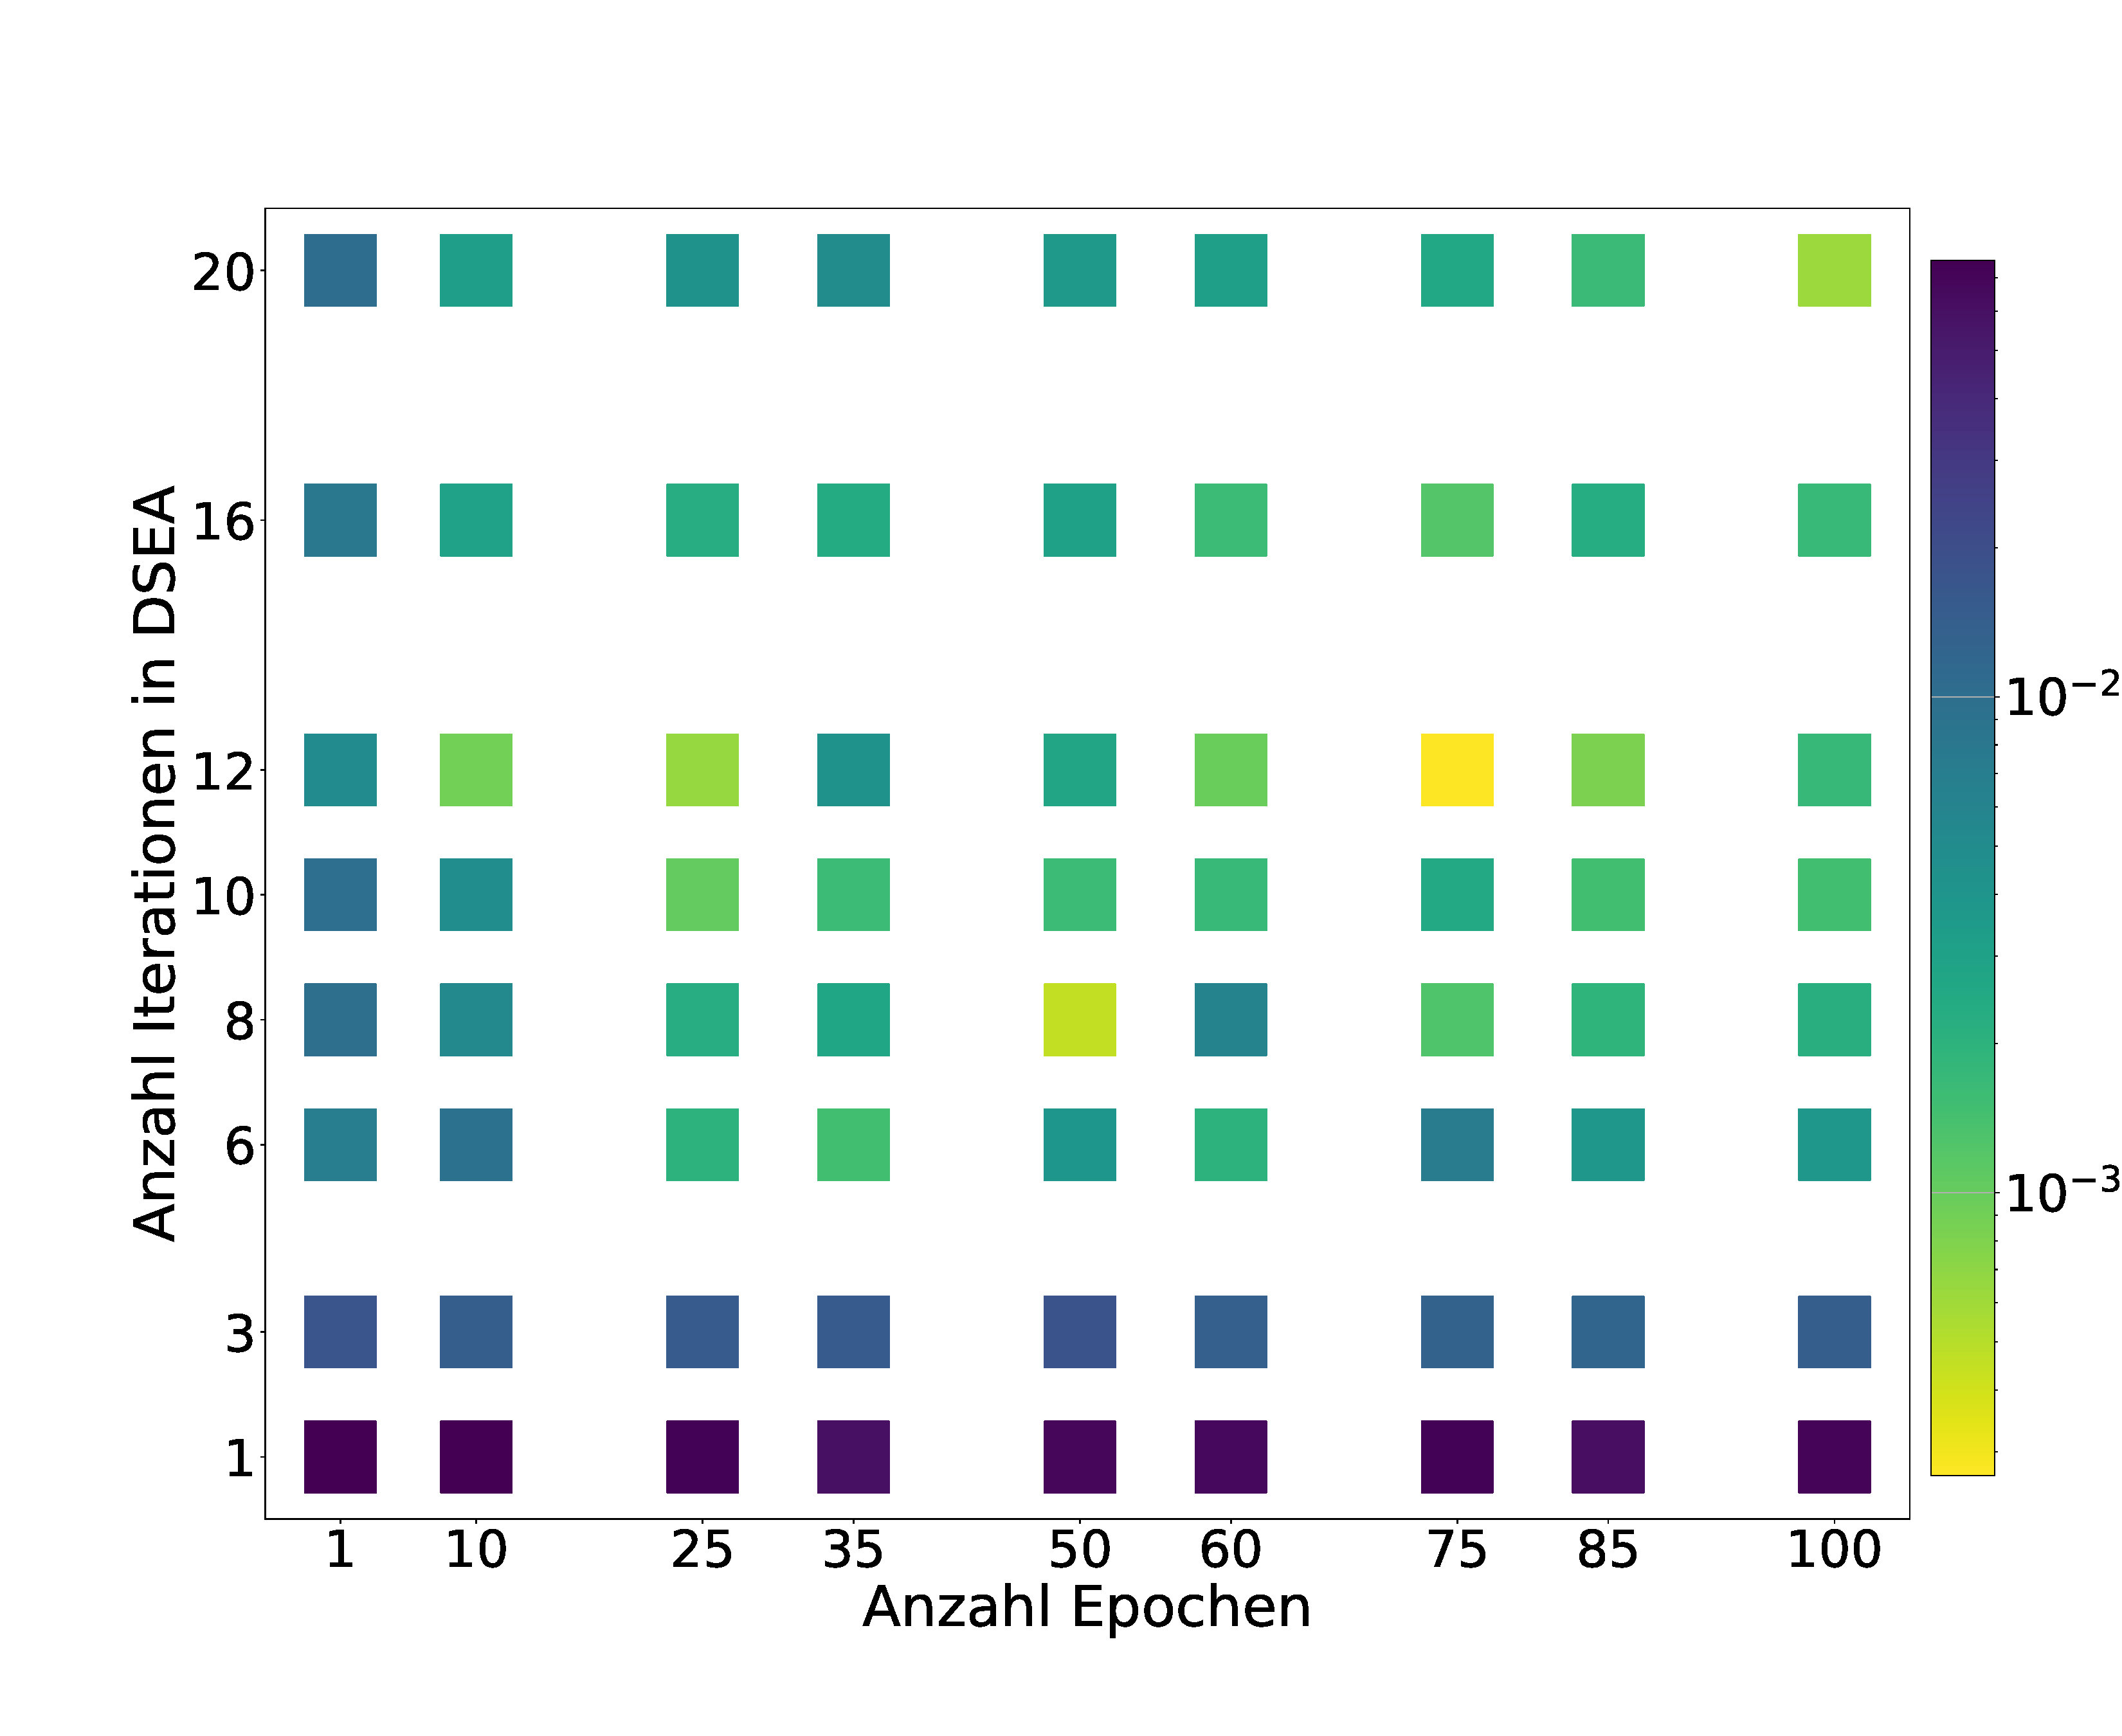
\includegraphics[width=1\textwidth]{Plots/DSEA/False/scatter_chi2.pdf}
    \caption[Ergebnisse der Gittersuche für mehrere (Anzahl: $n_\text{Iterationen}$) NN in DSEA]{Streudiagramm zur Darstellung der Ergebnisse der Gittersuche für Modell 1 (one\_model=False).
    In jeder DSEA-Iteration wird ein neues Modell erstellt und der Trainingsprozess beginnt von vorne.
    Die logarithmische Farbskala gibt den $\Chi^2$-Abstand zwischen dem wahren und vorhergesagten Spektrum an.
    }
    \label{fig:scatter_false}
\end{figure}

% trainings history: model 1 (one_model=False)
\begin{figure}%
    \begin{subfigure}{0.5\textwidth}%
        \centering%
        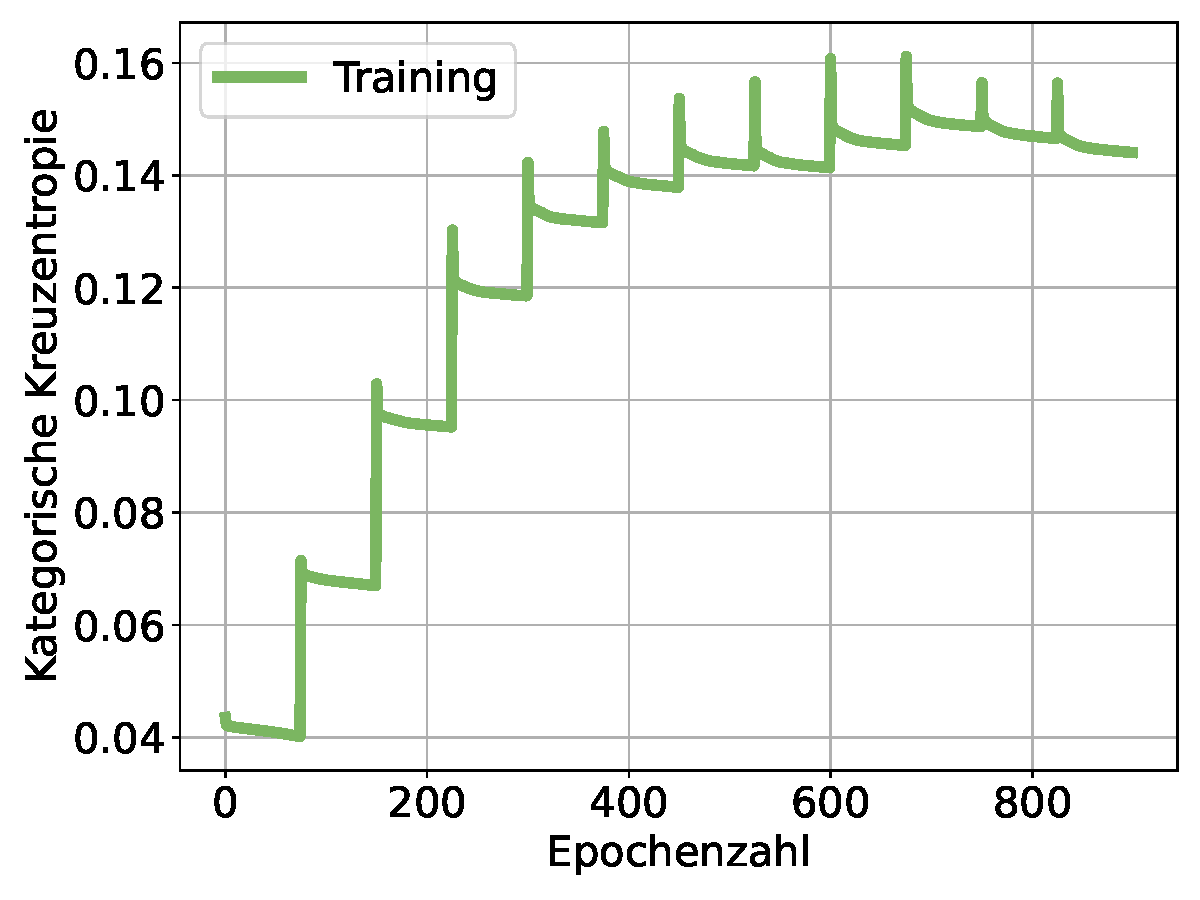
\includegraphics[height=5cm]{Plots/DSEA/False/loss.pdf}%
        \caption{Kostenfunktion: Kategorische Kreuzentropie}%
        %\label{fig:NN_loss}%
    \end{subfigure}%
    \hfill% Fills available space in the center -> space between figures
    \begin{subfigure}{0.5\textwidth}%
        \centering%
        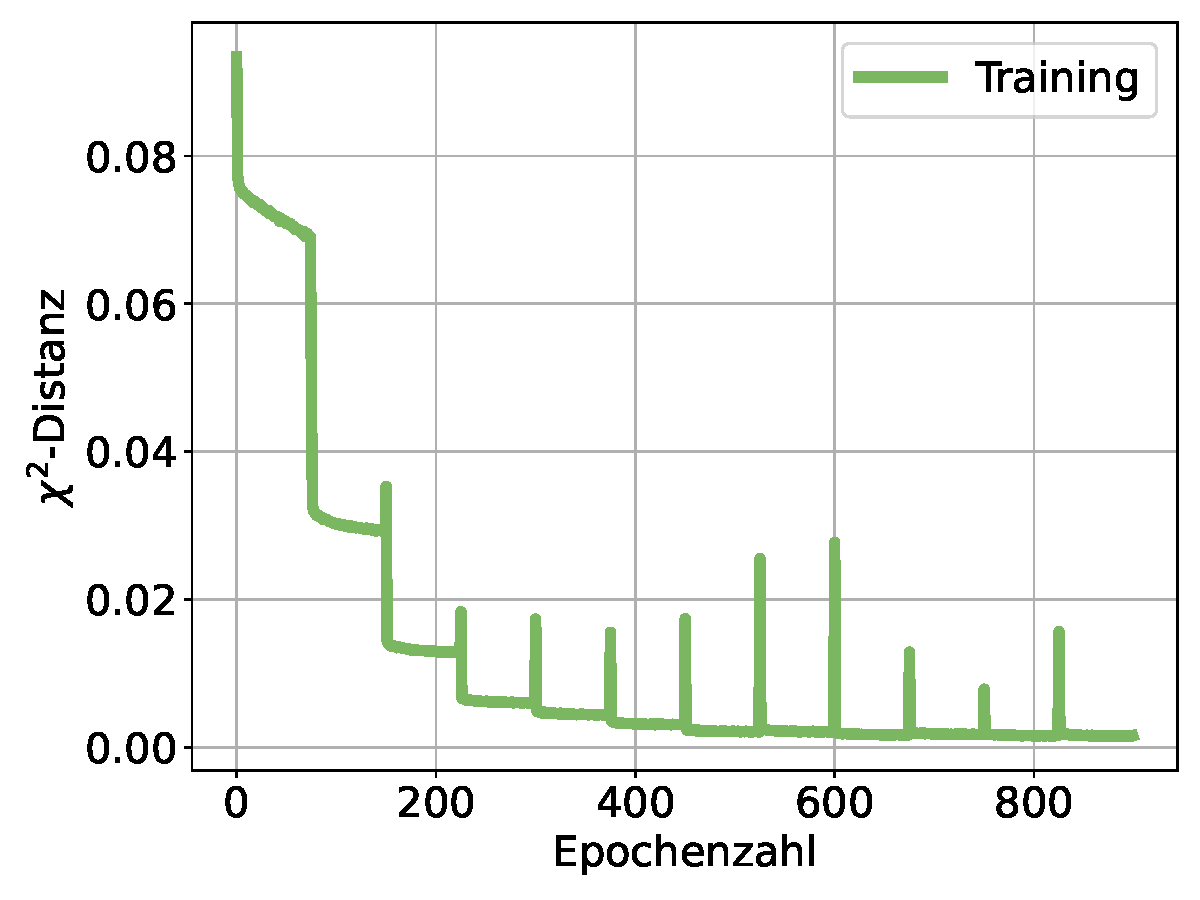
\includegraphics[height=5cm]{Plots/DSEA/False/chi.pdf}%
        \caption{Metrik: $\Chi^2$-Distanz}%
        %\label{fig:NN_chi}%
    \end{subfigure}%
    \caption[Verlauf des Trainingsprozesses des 1. Modells in DSEA]{Verlauf des Trainingsprozess des 1. Modells mit dem Parameter one\_model=False.
    In jeder DSEA-Iteration wird ein neues Modell mit aktualisierten Gewichten trainiert.
    Zum einen ist die Kostenfunktion \textit{kategorische Kreuzentropie} und zum anderen die \textit{Chi-Quadrat-Distanz} als Metrik in Abhängigkeit der Epochenzahl aufgeführt.
    }
    \label{fig:dsea_history_false}%
\end{figure}%}

% spectrum: model 1 (one_model=False)
\begin{figure}
    \centering
    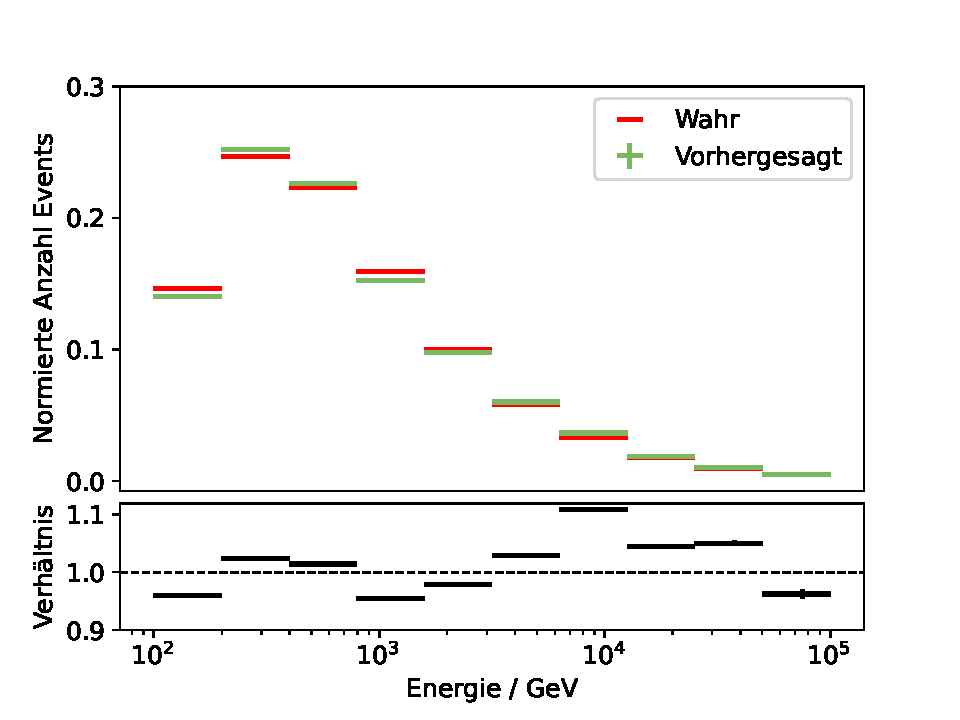
\includegraphics[width=0.9\textwidth]{Plots/DSEA/False/spectrum_dist_10bins_75ep_500000samples_200pulls.pdf}
    \caption[Spektrum des 1. Modells in DSEA]{Das entfaltete Spektrum des 1. Modells mit dem Parameter \textit{one\_model=False} und der zugehörige Verhältnis-Plot.
    In jeder DSEA-Iteration wird ein neues Modell mit aktualisierten Gewichten trainiert.
    }
    \label{fig:dsea_spectrum_false}
\end{figure}

% bootstrap: model 1 (one_model=False)
\begin{figure}%
    \centering%
    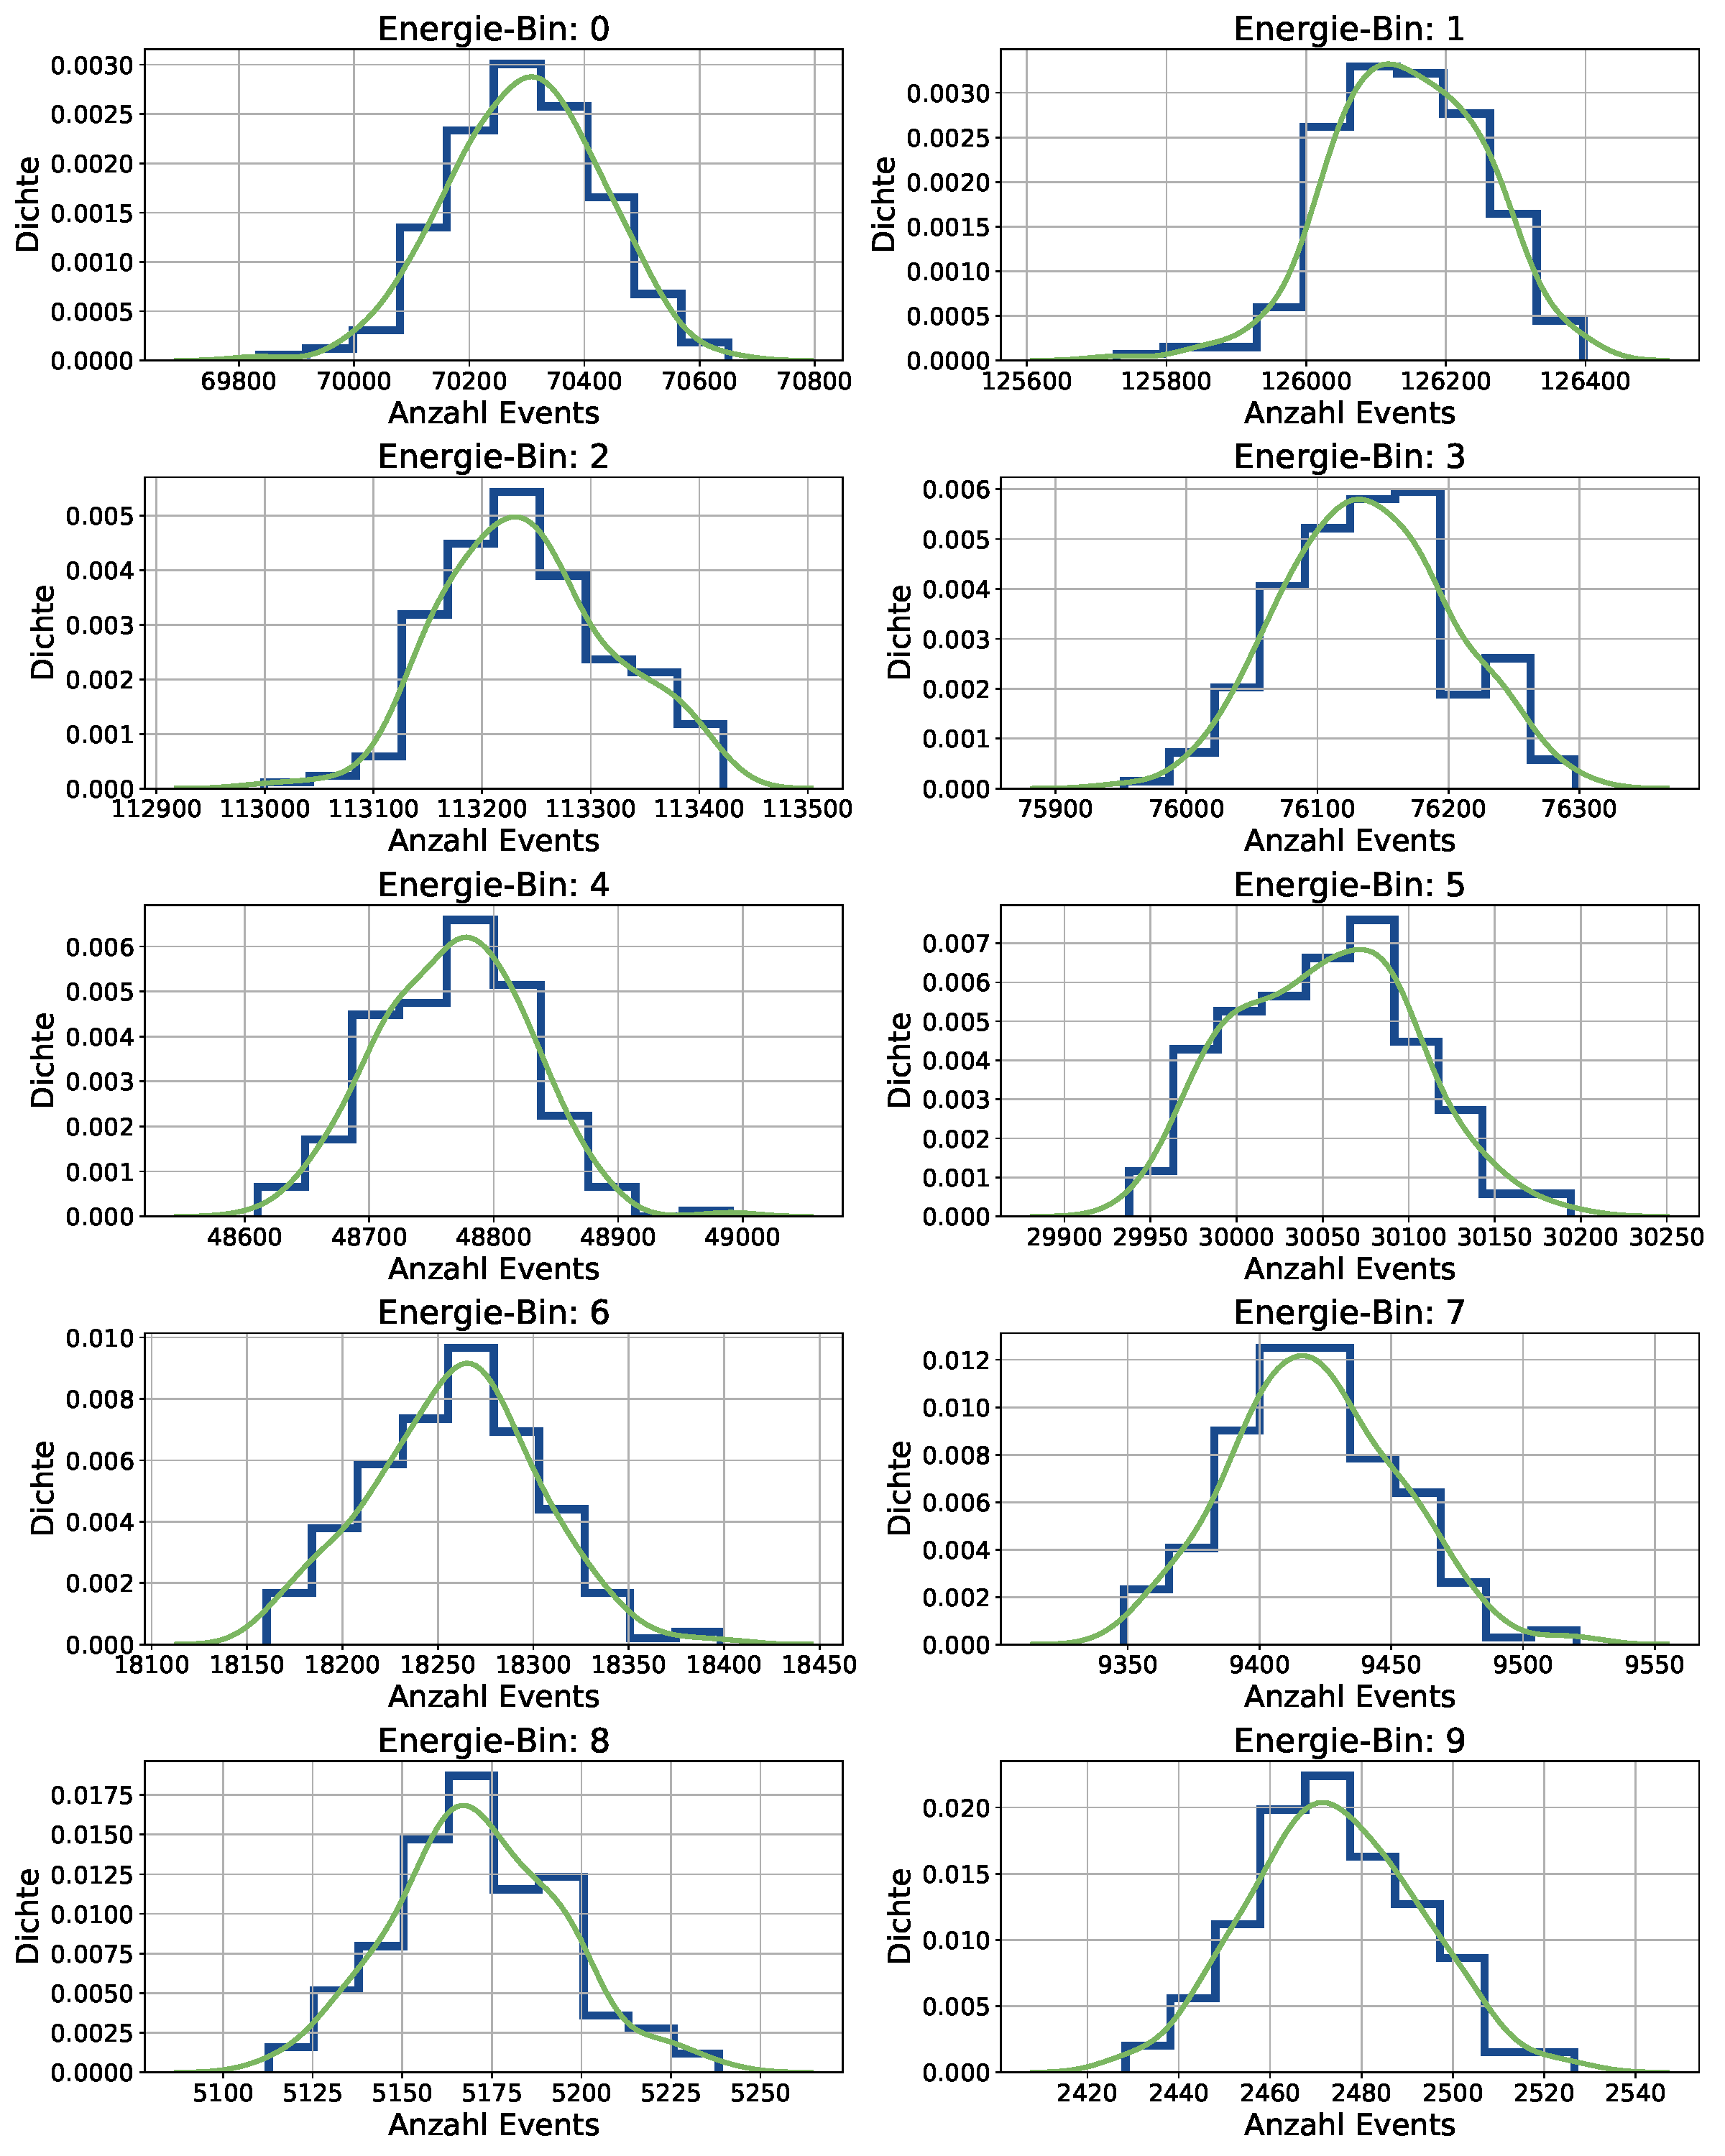
\includegraphics[width=\textwidth]{Plots/DSEA/False/class_dist_10bins_12it_75ep_500000samples_200pulls.pdf}%
    \caption[Ergebnisse des Bootstrapping-Vefahrens für das 1. Modell in DSEA]{Das blaue Histrogramm stellt die Verteilung der Bootstrap-Ergebnisse für Modell 1 (\textit{one\_model=False}) mit 200 Iterationen dar.
    Die rote Funktion repräsentiert einen Kerndichteschätzer(KDE) mit Gaußkern.
    Die Bin-Höhe wird durch den Median angegeben.
    Über das untere und obere Quantil werden die Unsicherheiten bestimmt.
    }%
    \label{fig:dsea_bootstrap_false}%
\end{figure}%

% bootstrap: model 2 (one_model=True)
\begin{figure}%
    \centering%
    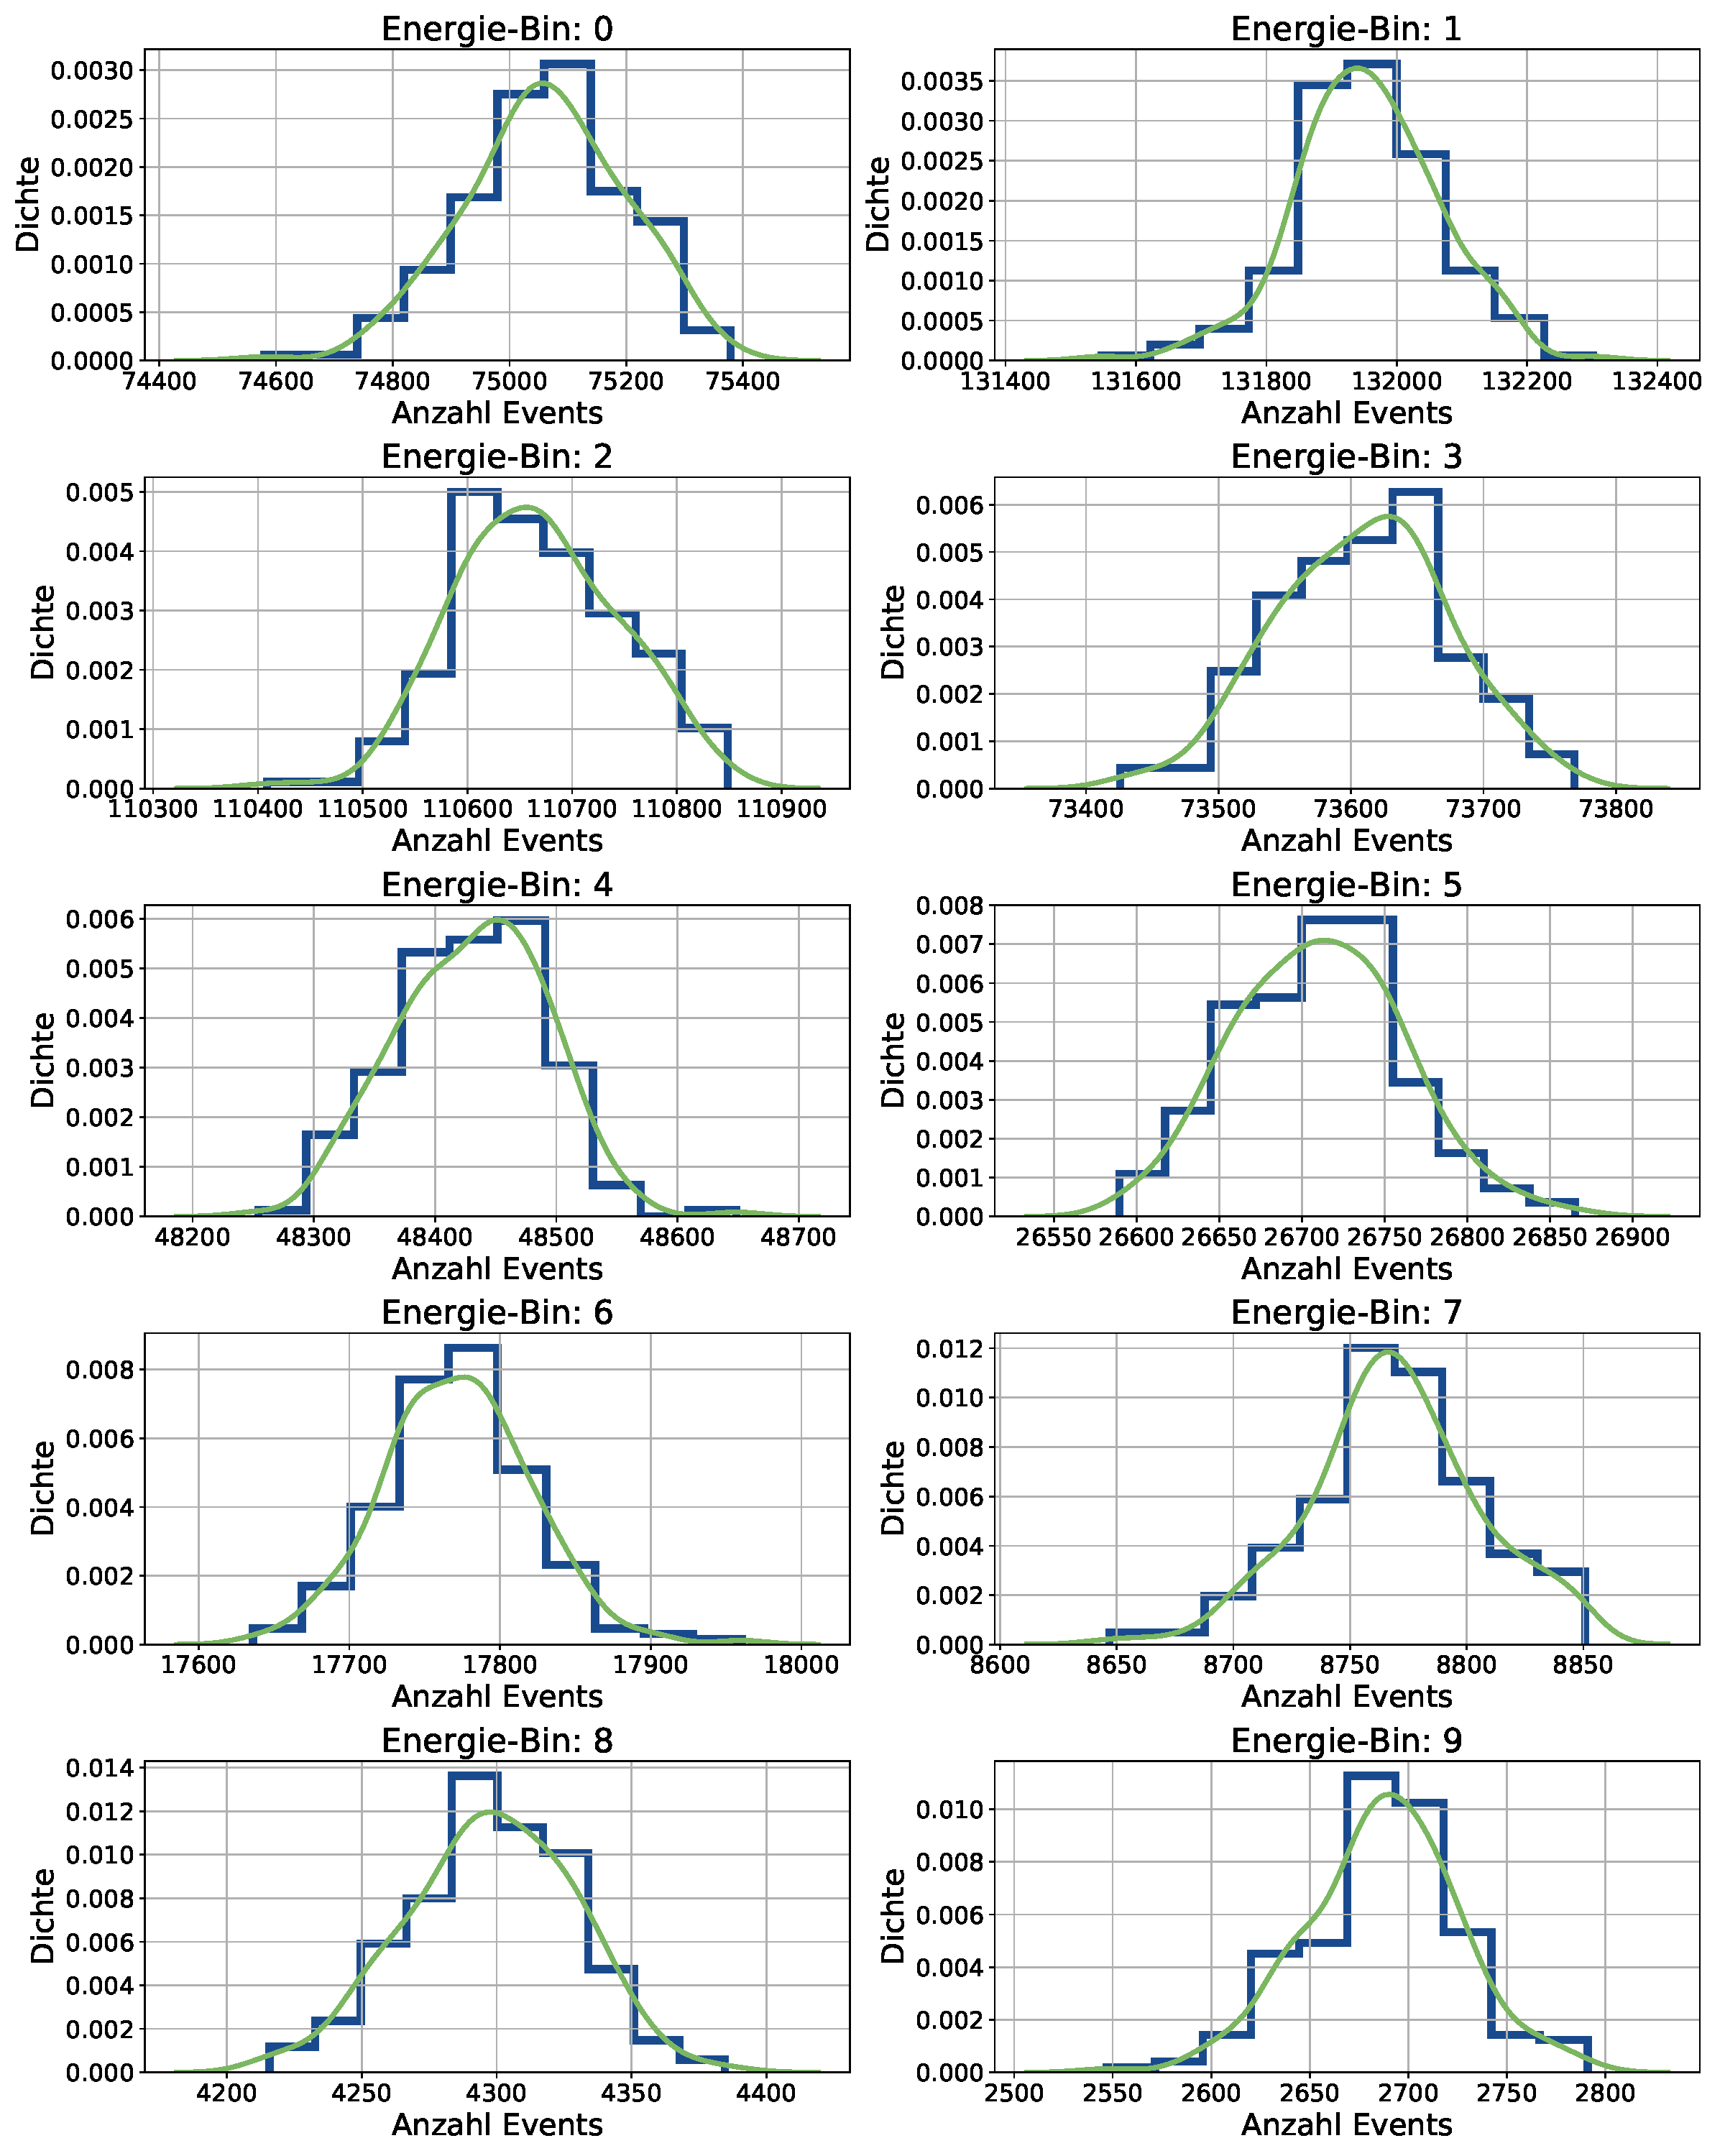
\includegraphics[width=\textwidth]{Plots/DSEA/True/class_dist_10bins_16it_60ep_500000samples_200pulls.pdf}%
    \caption[Ergebnisse des Bootstrapping-Vefahrens für das 2. Modell in DSEA]{Das blaue Histrogramm stellt die Verteilung der Bootstrap-Ergebnisse für Modell 2 (\textit{one\_model=True}) mit 200 Iterationen dar.
    Die rote Funktion repräsentiert einen Kerndichteschätzer(KDE) mit Gaußkern.
    Die Bin-Höhe wird durch den Median angegeben.
    Über das untere und obere Quantil werden die Unsicherheiten bestimmt.
    }%
    \label{fig:dsea_bootstrap_true}%
\end{figure}%

% single events: model 1(one_model=False)
\begin{figure}%
    \centering%
    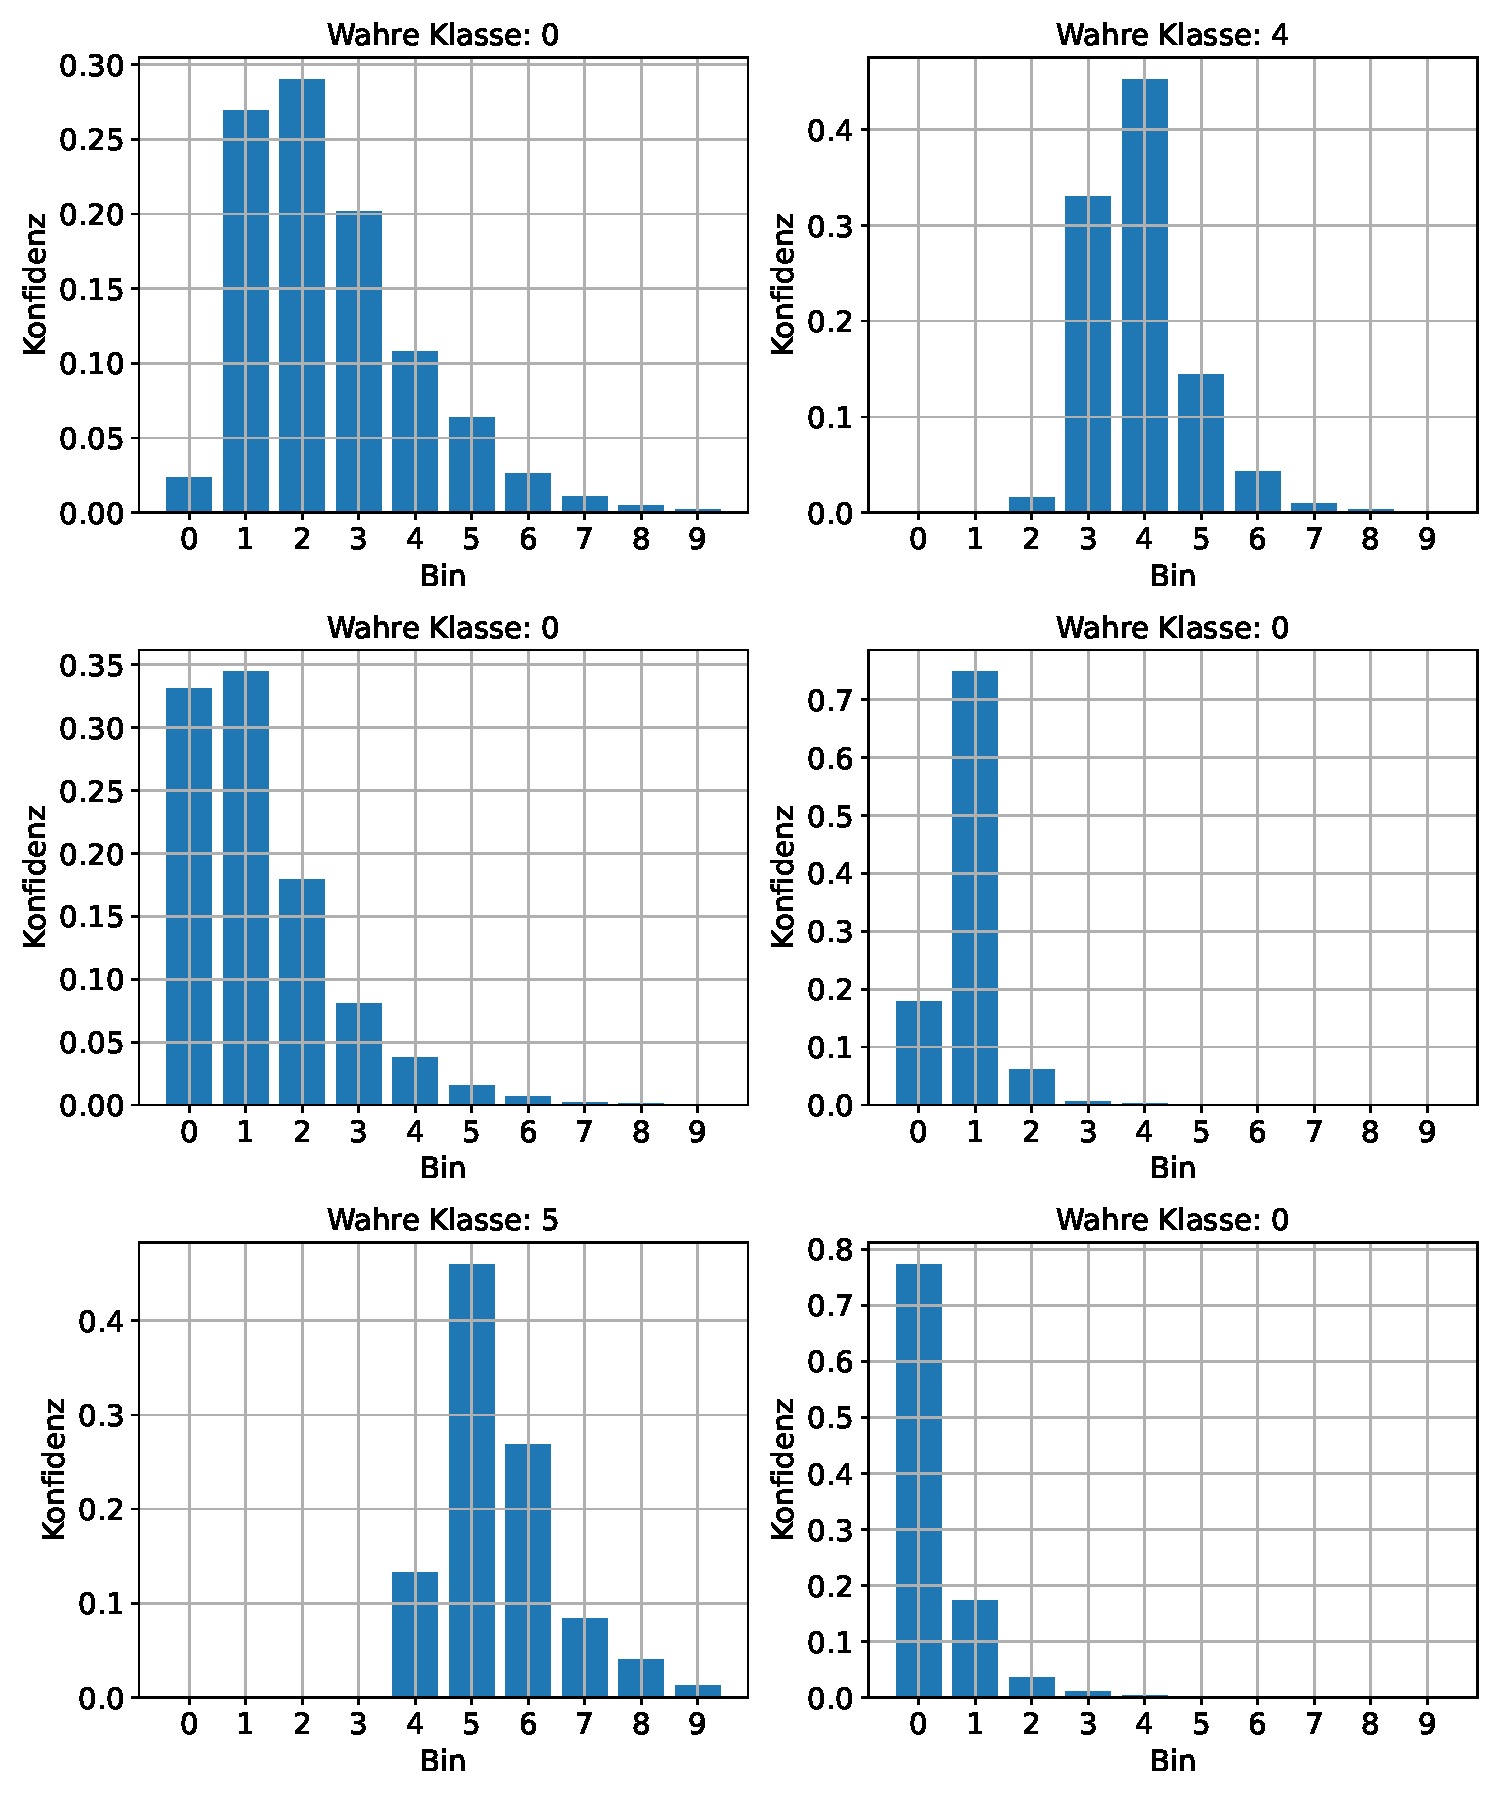
\includegraphics[width=\textwidth]{Plots/DSEA/False/SingleEvents_10bins_75ep_500000samples_200pulls.pdf}%
    \caption[Vorhersage einzelner Events des 1. Modells in DSEA]{Vorhersage einzelner Events des 1. Modells (\textit{one\_model=False}).
    Jedem Energie-Bin wird eine Konfidenz zugewiesen.
    Sie gibt die Zugehörigkeit des Events zu diesem Bin an.
    }%
    \label{fig:dsea_single_events_false}%
\end{figure}%

% single events: model 2(one_model=True)
\begin{figure}%
    \centering%
    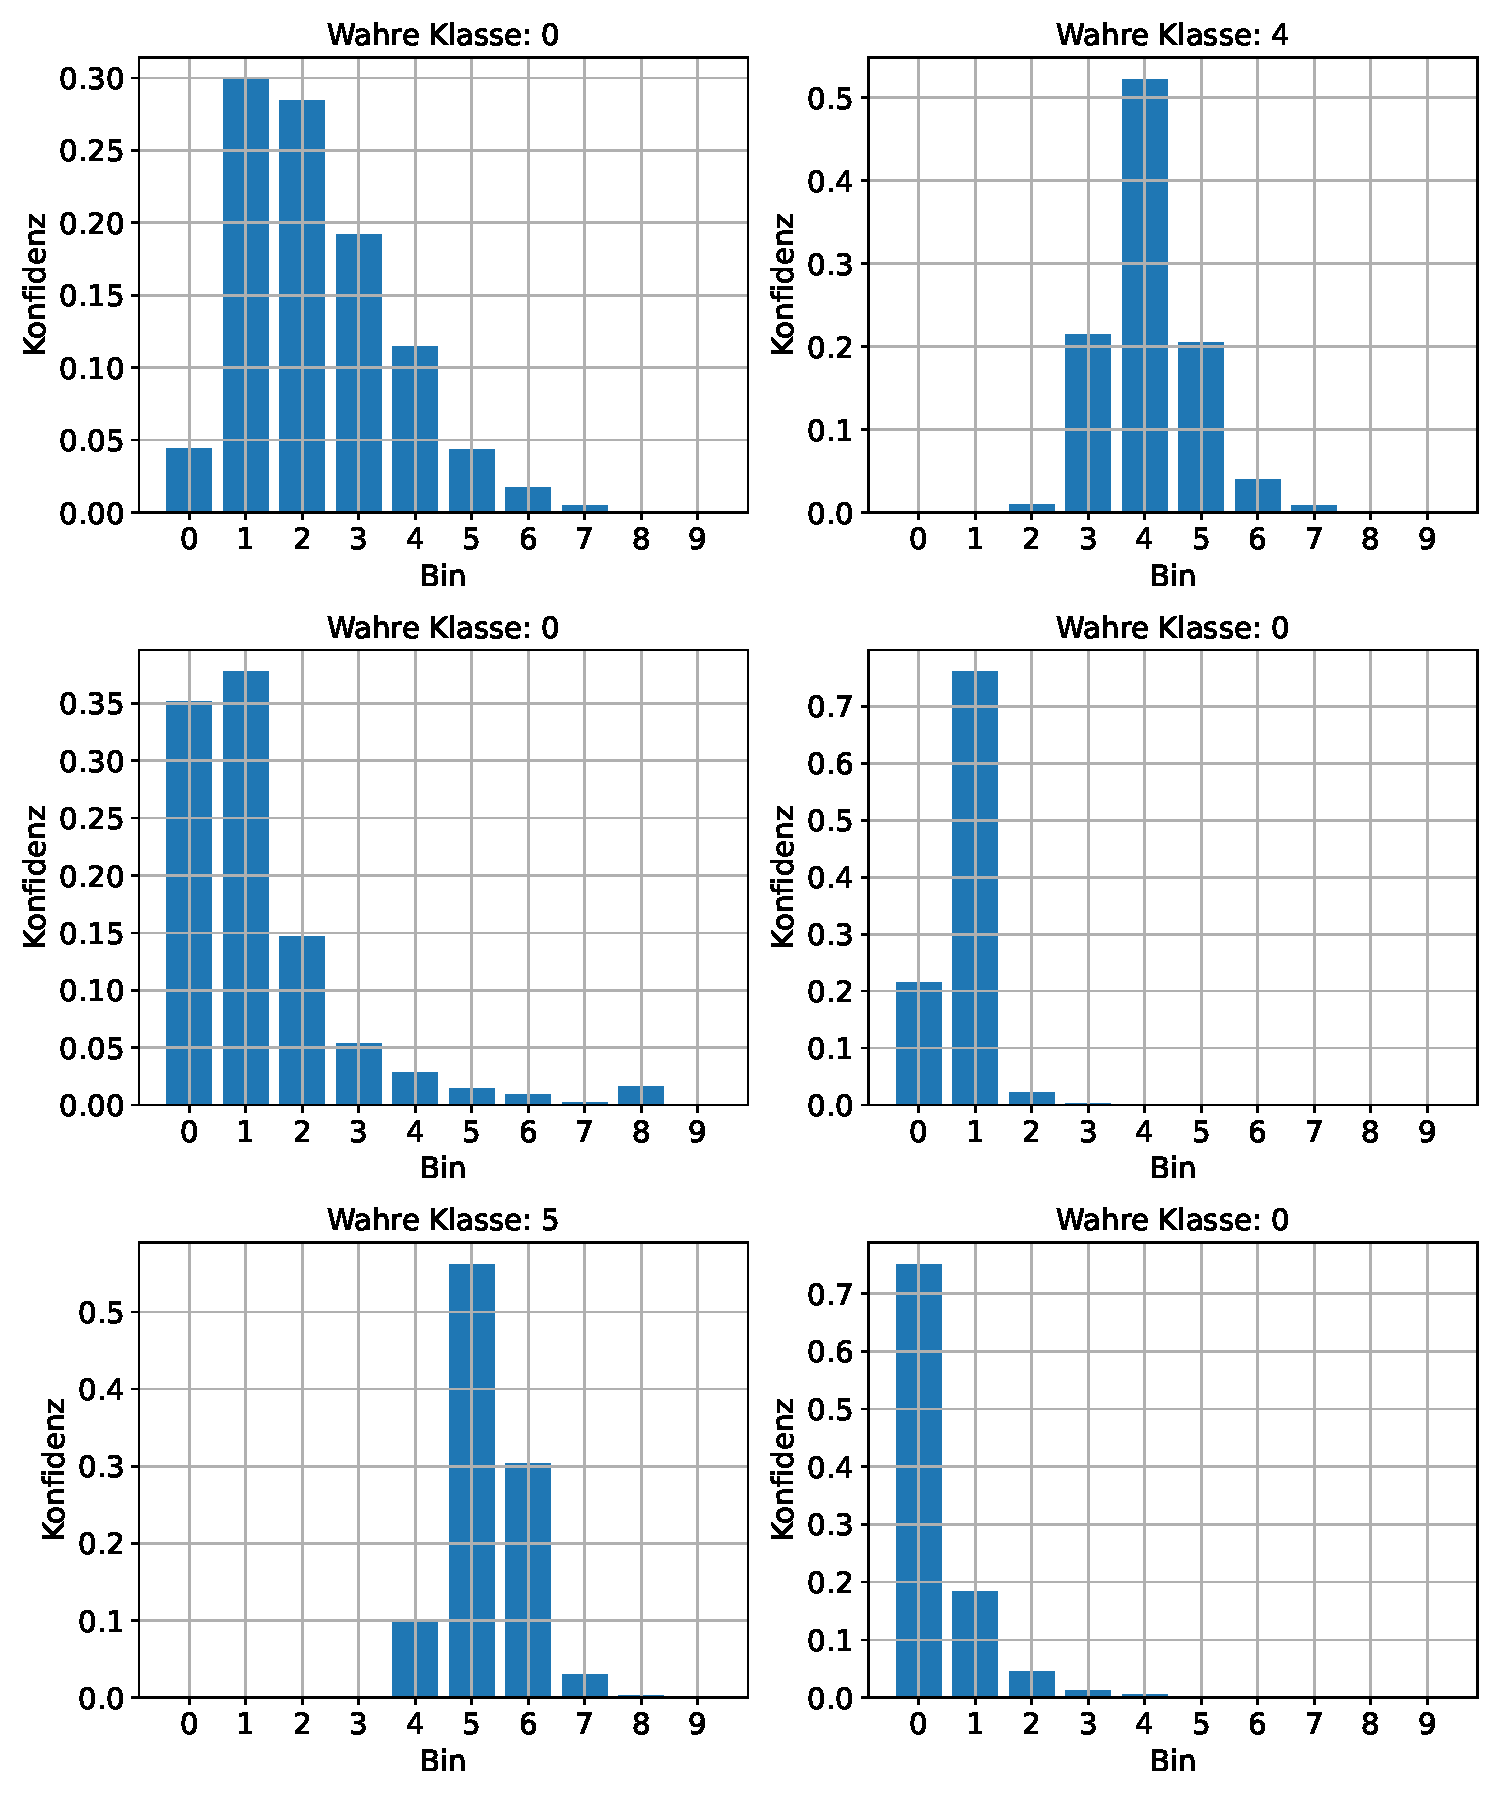
\includegraphics[width=\textwidth]{Plots/DSEA/True/SingleEvents_10bins_60ep_500000samples_200pulls.pdf}%
    \caption[Vorhersage einzelner Events des 2. Modells in DSEA]{Vorhersage einzelner Events des 2. Modells (\textit{one\_model=True}).
    Jedem Energie-Bin wird eine Konfidenz zugewiesen.
    Sie gibt die Zugehörigkeit des Events zu diesem Bin an.
    }%
    \label{fig:dsea_single_events_true}%
\end{figure}

% correlation matrix: model 1 (one_model=True)
\begin{figure}
    \centering
    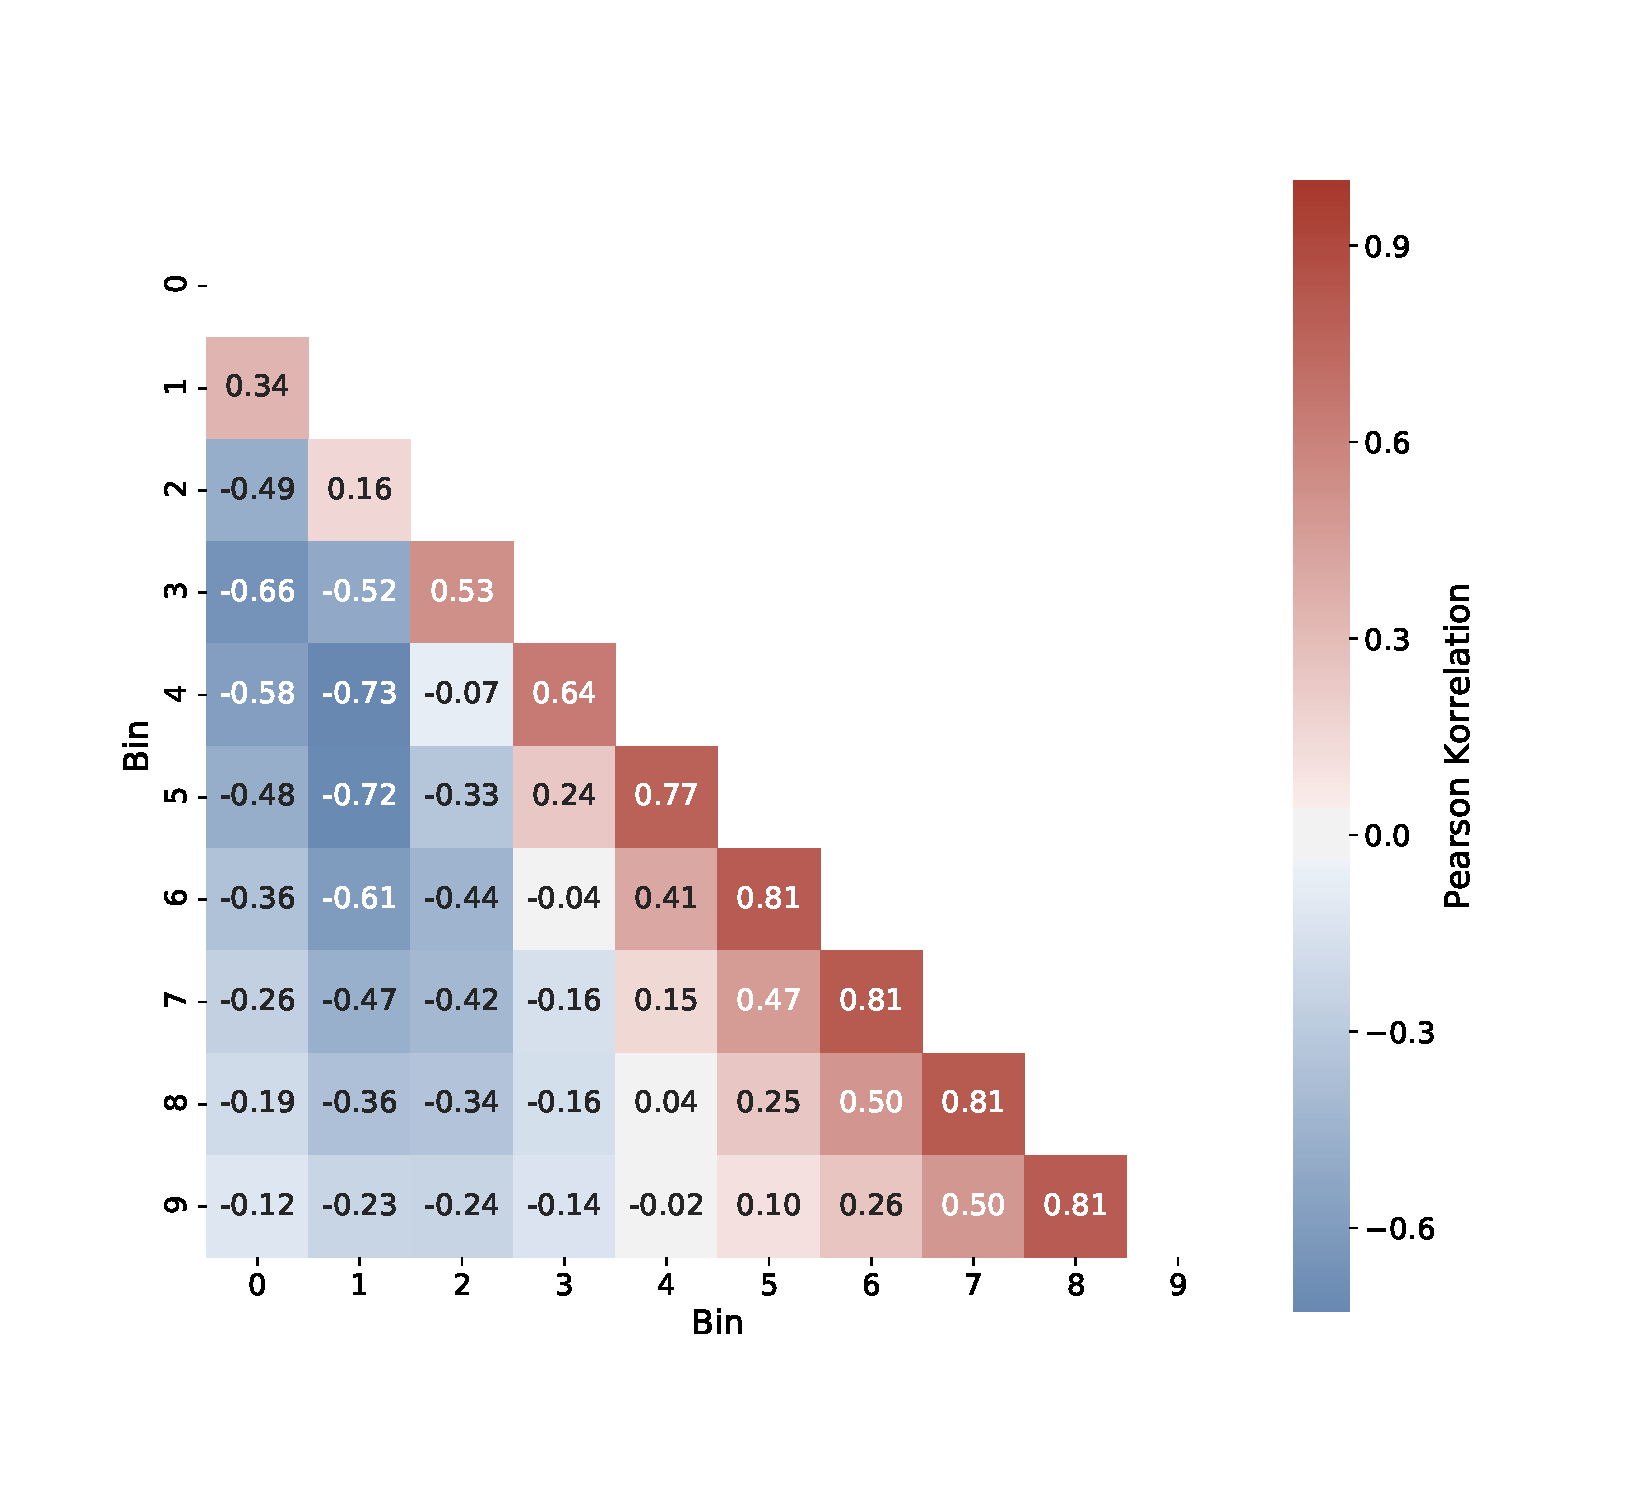
\includegraphics[width=1\textwidth]{Plots/DSEA/False/correlation_matrix.pdf}
    \caption[Korrelationsmatrix des 1. Modells in DSEA]{Die Korrelationsmatrix gibt die Korrelationen zwischen den entfalteten Energie-Bins an.
    Es handelt sich um das 1. Modell (\textit{one\_model=False}).
    }
    \label{fig:dsea_correlation_false}
\end{figure}